%%%% using 'arara' 4.0
% arara: xelatex: {synctex: yes, interaction: nonstopmode}
% arara: bibtex
% arara: xelatex: {synctex: yes, interaction: nonstopmode}
% arara: xelatex: {synctex: yes, interaction: nonstopmode}

% arara: indent: {overwrite: yes}

% arara: clean: { extensions: [aux, bcf, cod, blg, lof, lot, out, toc, log, xml, bak0 ] }

\documentclass[review]{elsarticle}

% Figures Links, mittig und rechts platzieren
\usepackage[export]{adjustbox}
\usepackage{caption}
\usepackage{subcaption}
\usepackage{amsmath}

\usepackage{enumerate}

% prevents that appendices are moved behind references
\usepackage{placeins}

\usepackage[nolist]{acronym}

\usepackage{longtable}
\usepackage{booktabs}
\usepackage{multirow}
\usepackage{float}

% https://tex.stackexchange.com/questions/165115/getting-not-defining-perthousnad-and-not-defining-micro-when-compiling-beamer
\usepackage{textcomp}

\graphicspath{{../03_figures/results/}{./}{../03_figures/data/}}

% enable paragraph as 4th level https://tex.stackexchange.com/questions/60209/how-to-add-an-extra-level-of-sections-with-headings-below-subsubsection
\usepackage{titlesec}
\setcounter{secnumdepth}{4}
\titleformat{\paragraph}
{\normalfont\small\bfseries}{\theparagraph}{1em}{}
\titlespacing*{\paragraph}
{0pt}{3.25ex plus 1ex minus .2ex}{1.5ex plus .2ex}

% enable linking to subsubsection
\setcounter{secnumdepth}{3}

% various symbols, e.g. \degree
\usepackage{gensymb}

\usepackage[hidelinks]{hyperref}

\usepackage{lineno}
\modulolinenumbers[5]

% set autoref abbr for appendix
\newcommand*{\Appendixautorefname}{appendix}

\journal{Journal "Remote Sensing of Environment"}

% line breaks in table cells
\newcommand{\specialcell}[2][l]{%
  \begin{tabular}[#1]{@{}l@{}}#2\end{tabular}}

% tilde
\newcommand{\mytilde}{\raise.17ex\hbox{$\scriptstyle\mathtt{\sim}$}}

%% APA style
\bibliographystyle{model5-names}\biboptions{authoryear}

\begin{document}

\begin{frontmatter}

	\title{Modeling defoliation as a proxy for tree health: A case study using machine-learning and hyperspectral remote sensing data}

	%% Group authors per affiliation:
	\author[FSU]{Patrick Schratz}
	\cortext[mycorrespondingauthor]{Corresponding author}
	\ead{patrick.schratz@uni-jena.de}

	\author[FSU]{Jannes Muenchow}
	\author[NEIKER]{Eugenia Iturritxa}
	\author[LMU]{Bernd Bischl}
	\author[FSU]{Alexander Brenning}

	\address[FSU]{Department of Geography, GIScience group, Grietgasse 6, 07743, Jena, Germany}
	\address[NEIKER]{NEIKER, Granja Modelo –Arkaute, Apdo. 46, 01080 Vitoria-Gasteiz, Arab, Spain}
	\address[LMU]{Department of Statistics, Chair for computational Statistics, Ludwig-Maximilian University Munich, Germany}

	\begin{abstract}

	\end{abstract}

	\begin{keyword}
		hyperspectral imagery \sep forest health modeling \sep machine-learning \sep feature-selection  \sep model comparison
	\end{keyword}

\end{frontmatter}

\linenumbers

% längste Abkürzung steht hier!!! in eckigen Klammern
\begin{acronym}[AUROC]

	% geringerer Zeilenabstand
	%\setlength{\itemsep}{-\parsep}
	\acro{AGB}{Above-Ground Biomass}
	\acro{ANN}{Artificial Neural Network}
	\acro{AUROC}{Area Under the Receiver Operating Characteristics Curve}
	\acro{BRT}{Boosted Regression Trees}
	\acro{CART}{Classification and Regression Trees}
	\acro{CV}{cross-validation}
	\acro{ENM}{Environmental Niche Modeling}
	\acro{FPR}{False Positive Rate}
	\acro{GAM}{Generalized Additive Model}
	\acro{GBM}{Gradient Boosting Machine}
	\acro{GLM}{Generalized Linear Model}
	\acro{ICGC}{Institut Cartografic i Geologic de Catalunya}
	\acro{IQR}{Interquartile Range}
	\acro{MARS}{Multivariate Adaptive Regression Splines}
	\acro{MEM}{Maximum Entropy Model}
	\acro{NDII}{Normalized Difference Infrared Index}
	\acro{NIR}{Near-Infrared}
	\acro{NRI}{Normalized Ratio Index}
	\acro{OLS}{Ordinary Least Squares}
	\acro{LOWESS}{Locally Weighted Scatter Plot Smoothing}
	\acro{PISR}{Potential Incoming Solar Radiation}
	\acro{RBF}{Radial Basis Function}
	\acro{RF}{Random Forest}
	\acro{RMSE}{Root Mean Square Error}
	\acro{RR}{Ridge Regression}
	\acro{RSS}{Residual Sum of Squares}
	\acro{SAR}{Synthetic Aperture Radar}
	\acro{SDM}{Species Distribution Modeling}
	\acro{SMBO}{Sequential-based Model Optimization}
	\acro{SVM}{Support Vector Machine}
	\acro{TPR}{True Positive Rate}
\end{acronym}

\section{Introduction}
\label{sec:intro}

% Explain how remote sensing is used in forestry (potential to map forest health)
% Link remote sensing and machine-learning
The use of machine-learning algorithms for analyzing remote sensing data has seen a huge increase in the last decade.
Ever since the launch of the first Sentinel satellite in 2014 the amount of freely available imagery data has increased enormously (REF).
At the same time, the implementation of algorithms (both statistical and machine-learning) has been greatly simplified in the open-source community.
Scientists can nowadays relively easily feed large amounts of data into complex algorithms in a semi-automated way.
These facts combined with a high temporal and spatial coverage of input data enable the possibility to analyze temporal changes of the environment on a large scale.

% link to forest health analysis and show exemplary studies
The monitoring of forest ecosystems is one exemplary field that profits from these new possibilities.
Specifically the monitoring of forest health got simplified with the ability of analyzing large scale data in efficient algorithms that are able to predict to unknown areas.
For this task, usually optical data from multi-/hyperspectral satellites is used.
Various indices are calculated from the data with the aim of carrying out temporal change detections \citep{zhang2016} or analyses about the forest health status for a specific date \citep{townsend2012}.
% TODO: check if refs match context
Vegetation indices have shown the potential to provide valuable information for analyzing triggers to forest health \citep{jiang2014, adamczyk2015}.
More and more studies focus on using machine-learning algorithms such as \ac{RF} \citep{belgiu2016, lary2016, michez2016}.
Overall, the idea is to fit a robust model which can be used to make predictions to (large) unknown areas, providing valuable information about the health condition of forest stands without the need for ground-truth data in these regions.

% now mention why this study is important
However, we have the impression that the amount of (vegetation-)indices used in forest health studies could be higher, possibly leading to more valuable results.
Possible reasons include the low spectral resolution of optical multispectral sensors, the lack of freely available hyperspectral data or the lack of knowledge about existing indices.
% TODO: Ref for high-dim
Another more applied issue is the fact of high-dimensionality which is introduced by the calculation of hundreds/thousands of indices.
% TODO: Ref model interpr
Even though ML algorithms are capable of handling possibly highly-correlated input variables, model runtime increases substantially and the interpretation of results becomes more complicated.
Also, in recent years the awareness of conducting proper tuning of model hyperparameters has increased in applied modelling fields.
In this study we addressed these challenges by focusing on the following research questions:

\begin{itemize}
	\item How to handle and analyze high-dimensional data including model optimization while accounting for spatial characteristics?
	\item Does the calculation of arbitrary indices add any value to the analysis or is the band information from the sensor already sufficient?
	\item How can interpretability of the model be maintained while at the same time using all possible input data?
\end{itemize}

\noindent State-of-the-art machine-learning techniques were compared using three feature sets across different feature-selection approaches including a relatively novel approach of ensemble filters.
To model the numeric response variable defoliation at trees model-based optimization was applied for hyperparameter tuning and a spatial block \ac{CV} was used to account for spatial autocorrelation in the data.

\section{Data and study area}
\noindent Airborne hyperspectral data with a spatial resolution of one meter and 126 spectral bands was available for four Monterey Pine (\textit{Pinus radiata}) plantations in northern Spain (\autoref{fig:study_area}).
The trees in the study area plots suffer from infections of invasive pathogens such as \textit{Diplodia sapinea}, \textit{Fusarium circinatum}, \textit{Armillaria mellea} or \textit{Heterobasidion annosum} leading to a spread of cankers or defoliation \citep{mesanza2016, iturritxa2017}.
In-situ measurements of defoliation at trees (as a proxy for tree health) were collected to serve as the response variable \textit{defoliation} spanning a range from 0\% - 100\%.
The fungi are assumed to infect the trees through open wounds, possibly caused by previous hail damage \citep{iturritxa2014}.
The dieback of these trees, which are mainly used as timber, causes high economic damages \citep{ganley2009}.

\subsection{In-situ data}

\noindent The \textit{Pinus radiata} plots of this study, namely \textit{Laukiz 1}, \textit{Laukiz 2}, \textit{Luiando} and \textit{Oiartzun}, are located in the northern part of the Basque Country (\autoref{fig:study_area}).
\textit{Oiartzun} has the most observations (n = 529) while \textit{Laukiz 2} features the largest area size (1.44 ha).
All plots besides \textit{Luiando} are located nearby the coast (\autoref{fig:study_area}).
In total 1750 observations are available (\textit{Laukiz 1} = 479, \textit{Laukiz 2} = 451, \textit{Luiando} = 291, \textit{Oiartzun} = 529).
The data was surveyed in September 2016.

%\begin{figure} [t!]
%\begin{center}
%\makebox[\textwidth]{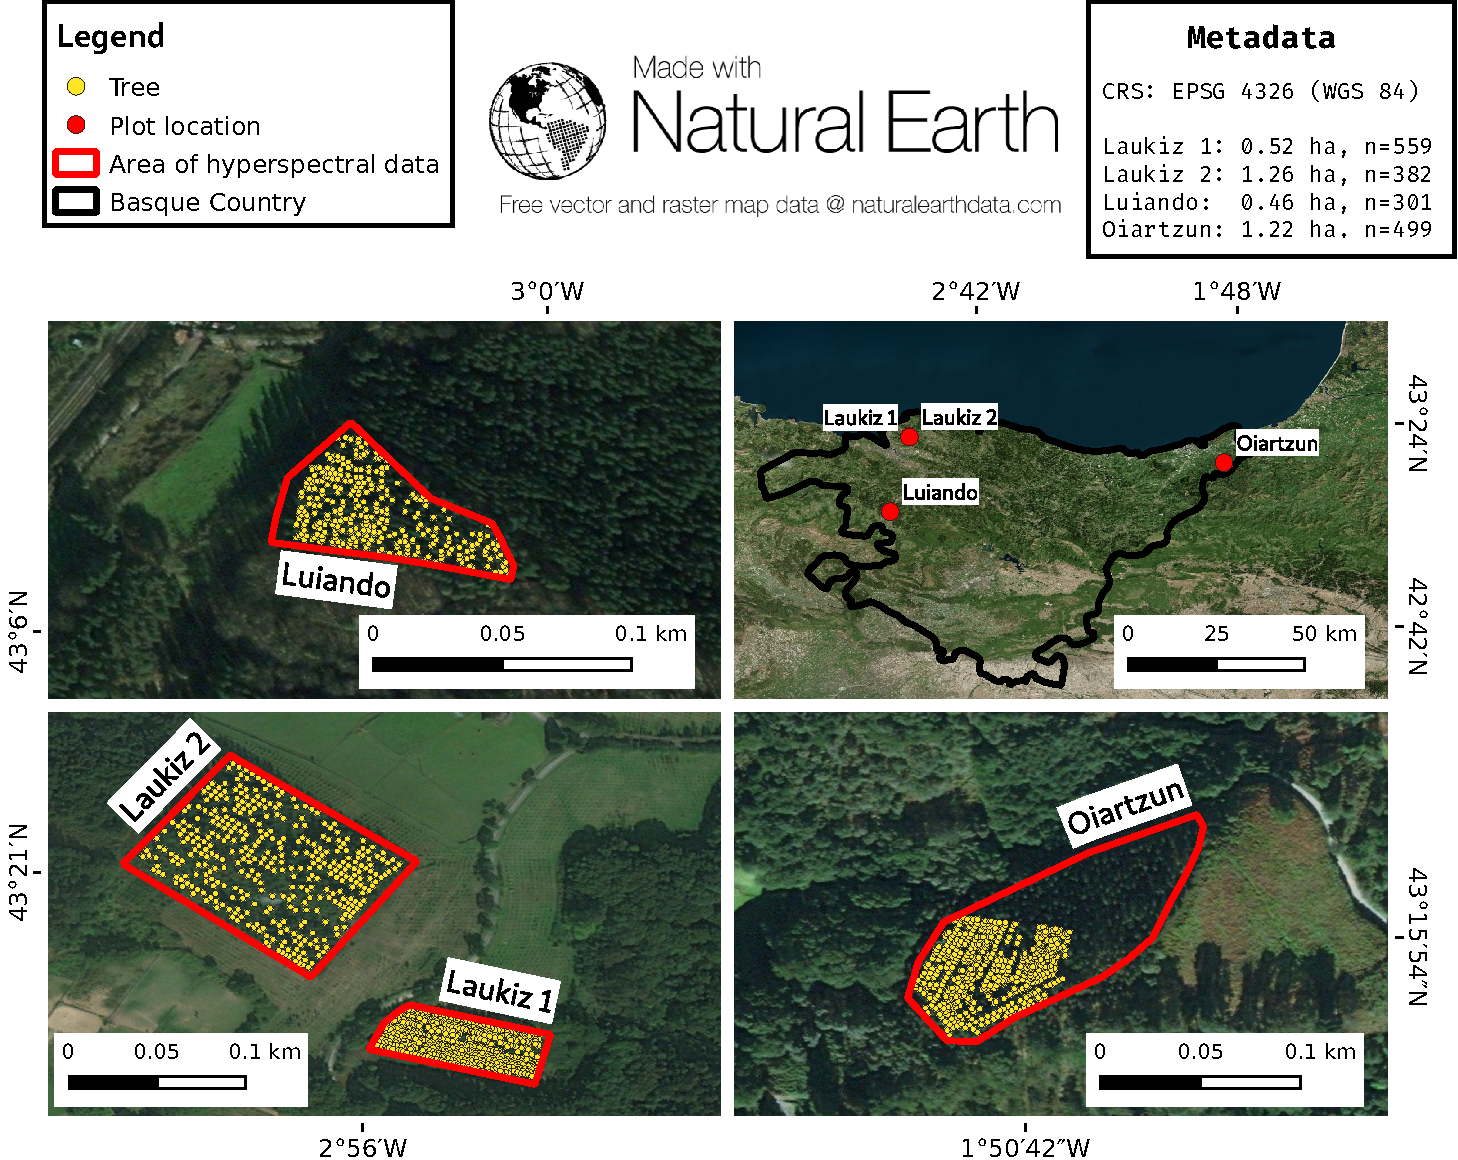
\includegraphics[width=\textwidth] {study_area_hyperspectral.pdf}}
%\caption{Information about the plot locations, the area of hyperspectral coverage and the number of trees per plot.}
%\label{fig:study_area}
%\end{center}
%\end{figure}


\subsection{Hyperspectral data}

\noindent The airborne hyperspectral data was acquired during two flight campaigns on September 28th and October 5th 2016, both around 12 am.
The images were taken using a AISAEAGLE-II sensor.
All preprocessing steps (geometric, radiometric, atmospheric) have been conducted by the \ac{ICGC}.
The first four bands are corrupted, leaving 122 bands with valid information.
Additional metadata information is available in \autoref{tab:hyperparameter_limits}.

% parameter limits
\begin{table}[b!]
\centering
\caption[t]{Specifications of hyperspectral data.}
\begingroup\footnotesize
\begin{tabular}{ll}
	\\
	Characteristic         & Value                               \\
	\hline
	Geometric resolution   & 1 m                                 \\
	Radiometric resolution & 12 bit                              \\
	Spectral resolution    & 126 bands (404.08 nm - 996.31 nm)   \\
	Correction:            & Radiometric, geometric, atmospheric
\end{tabular}
\endgroup
\label{tab:hyperparameter_limits}
\end{table}



\section{Methods}

\subsection{Derivation of indices}
% TODO: Mention different feature sets
\noindent To use the full information from the hyperspectral data, all possible vegetation indices supported by the \textit{hsdar} package (90 in total) as well as all possible \ac{NRI} combinations were calculated.
The following formula was used for the NRI calculation:

\begin{equation}
	NRI_{i,j} = \frac{b_{i} - b_{j}}{b_{i} + b_{j}}
\end{equation}

\noindent
where $i$ and $j$ are the respective band numbers.

\bigbreak

\noindent To account for geometric offsets (which were reported with up to 1 m from \ac{ICGC}), a buffer of two meters around the centroid of the respective tree was used.
The mean of all pixels touched by this buffer was calculated and assigned to the observations.
In total, $\frac{125*126}{2} = 7875$ NRIs were calculated .
Due to four corrupted bands and numerical calculation errors for some band combinations, a total of 7471 indices was available for each observation.
If an index returned \texttt{NA} for one plot, the index was removed from all plots.
This decision was based on the fact that due to the mass of available indices and the low number of observations, the latter was valued higher.

\subsection{Benchmarking design}

The benchmarking matrix of this study consists of the following algorithms:

\begin{itemize}
	\item  Extreme Gradient Boosting (\ac{XGBOOST})
	\item  Random Forest (\ac{RF})
	\item  Penalized Regression (both L1 and L2)
	\item  Support Vector Machine (\ac{SVM})
\end{itemize}

\ac{RF} and {SVM} are well established algorithms that are widely used in environmental modeling.
Extreme Gradient Boosting (commonly referred to as \ac{XGBOOST}) showed promising results in benchmark competitions in recent years.
Penalized Regression is a statistical modeling technique that is capable of dealing with highly-correlated covariates by applying a penalization term which shrinks the coefficients of the model.
The penalties are also known as LASSO (L1) and RIDGE (L2).
The former does not allow the removal of variables from the model (penalization to zero) while the latter does.
Both penalties can also be combined.
The combined approach is called "elastic net".

\subsubsection{Feature sets}

Three feature sets were used in this study:

\begin{itemize}
	\item The raw hyperspectal band information (HR, $n = 122$)
	\item Vegetation Indices (\ac{VI}, $n = 90$)
	\item Normalized Ratio Indices (\ac{NRI}, $n = 7471$)
\end{itemize}


\subsubsection{Hyperparameter Optimization}

An exhaustive hyperparameter tuning was applied during nested spatial \ac{CV} for all algorithms.
Maximum Bayesian Optimization \citep{mlrmbo} was used for parameter optimization.
This approach first composes \textit{n} randomly chosen hyperparameter settings out of a user defined search space.
After these \textit{n} tries have been evaluated, a new hyperparameter setting, which is going to be evaluated next, is proposed based on a fitted regression model.
The regression model estimates the performance of the machine-learning method for unknown hyperparameter settings.
Using these estimates, a new promising hyperparameter setting is proposed to be evaluated next.
This strategy continues until a termination criterion, defined by the user, is reached \citep{hutter2011, jones1998}.
An initial design of 30 randomly composed hyperparameter settings and a termination criterion of 70 iterations was used, resulting in a total budget of 100 evaluated hyperparameter settings per fold.
The advantage of this tuning approach is the substantial reduction of the tuning budget required to find a setting which is close to the global minimum
This applies when being compared to methods that do not use information from previous runs, such as random search or grid search \citep{bergstra2012}.

\subsubsection{Spatial resampling}

A spatial block nested cross-validation was chosen to reduce the influence of spatial autocorrelation as much as possible.
Each tree plot served as one fold within the resampling setup, resulting in four folds total.
For the inner level, $p - 1$ folds were used (with $p$ being the number of plots).

\subsection{Dealing with high-dimensionality}
% Define "high-dimensionality"
The usage of the term "high-dimensionality" in the machine-learning field practically means to deal with dataset that has a high amount of covariates.
There is no clear threshold at which number the term can be applied.
There has been an informal agreement to speak of "high-dimensonialty" if the number of variables exceeds the number of observations. REF

The case of a high-dimensional dataset comes with several challenges for both model fitting and evaluation.
There is an increase in time for fitting a model to the data.
Possible noise maybe introduced into the model by highly-correlated variables.
The interpretation and prediction of models containing hundreds of covariates becomes more complicated, up to to the point at which interpretation or prediction is not possible anymore.
Especially in the last decade the amount of data increased a lot and also the environmental modeling field profited from this as well.
Numerous approaches were developed to deal with this situation and the field of "feature selection" can be safely seen as a standalone research field.

\subsubsection{Filter methods}

% Filter methods
So called "Filter methods" are one approach.
The basic concept relies on the ranking of all features of the dataset using heuristics of the respective algorithm.
Some are tailored towards specific types of variables (numeric or nominal data).
After the covariates have been ranked, a decision needs to be made what features to keep and which to discard.
This step is usually done within the optimization phase of the model fitting, along with the hyperparameter tuning.
Essentially, the number of covariates in the model is treated as a hyperparameter of the respective model.
The goal is to find the threshold (usually in \% of covariates) at which the model achieves a good performance while requiring the least amount of variables.
In well-implemented software solutions the calculations of the ranking is only done once and then cached.
In subsequent tuning iterations the results are taken from the cache instead of being calculated again.

% Ensembe filter methods
Besides the idea of using single filter methods to rank variables, studies showed that combining several filters using statistical operations such as "minimum", "mean" or "sum" are able to enhance the predictive performance of the resulting models.
This aligns with the recent rise of the "ensemble" approach which was first used to combine the predictions of multiple models.
In this work we also used one ensemble filter method based on the "Borda" aggregation.
Here, the ranks of all single filters are summed up leading to a final ranking which consists of the ranks achieved by all filter algorithms.

Most filter methods are correlation or entropy based.
A list of all filter methods used in this work along with their respective formulas can be found in Appendix X.
% TODO: Link appendix
% TODO: List filter methods

\subsubsection{Other approaches}

% Wrapper approach
Another approach to reduce the number of variables is to apply algorithms that are normally used for hyperparameter optimization such as \textit{Random Search} or a \textit{Genetic Algorithm}.
Here, first a (random) subset of features is chosen based on the selected algorithm.
In comparison to "filters", no ranking is applied here.
Now the model is fitted on the data and the performance is evaluated.
A major downside of this approach is that hyperparameter tuning can only start after the feature-selection optimization has ended.
Hence, this method is very expensive because two optimization stages need to be run.
In science this approach is also referred to as "wrapper method".
It was not considered in this work due to the expensive runtime.

% PCA
A third commonly used method is the "Principal Component Analysis".
Here, the main components of the feature space are extracted and combined.
Usually the first two components are taken since these contain the major information of the covariates.
By using the (automatically estimated) explained variance of the main components, the model can rely on a few features containing the condensed information of most variables of the data.
This enables a very cheap model fitting with a minimal loss of predictor information.
However, the resulting features used in the model do not relate anymore to the raw input variables since they are a combination of multiple covariates.
Interpretation is not possible anymore.

\noindent The complete study was done using the open-source statistical programming language R \citep{rcoreteam2018}.
The algorithm implementations of the following packages have been used: \textit{xgboost} \citep{chen2016} (\textit{xgboost}), \textit{e1071} \citep{e1071} (Support Vector Machine) and \textit{glmnet} \citep{glmnet} (Ridge Regression).
The filter methods of the following packages were used: \textit{praznik}, \textit{fselectorrcpp}.
The R package \textit{mlr} \citep{mlr} was used for all modeling related steps.
\textit{drake} was used for structuring the work and ensuring reproducbility.
This study is available as a research compendium on Zenodo (\url{10.5281/zenodo.2635403}).

\section{Results}

\subsection{Plot characteristics}

%% defoliation boxplots
%\begin{figure} [t!]
%\begin{center}
%\makebox[\textwidth]{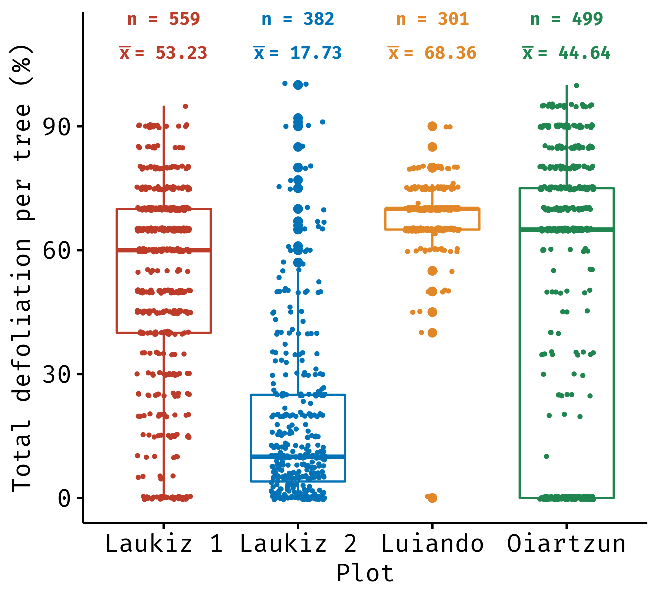
\includegraphics[width=0.7\textwidth] {boxplot_defol.pdf}}
%\caption{Descriptive statistics of the response variable \textit{defoliation}.}
%\label{fig:defol_boxplots}
%\end{center}
%\end{figure}

%\noindent \textit{Oiartzun} shows the highest defoliation ($\bar{x} = 69.22 \%$) among the plots while \textit{Laukiz 2} is the healthiest ($\bar{x} = 13.54 \%$) (\autoref{fig:defol_boxplots}).
%All plots besides \textit{Luiando} show an evenly distributed level of defoliation across the entire plot.

%\noindent The high degree of defoliation for \textit{Luiando} and \textit{Oiartzun} is also visible in the spectral signatures of the plots (\autoref{fig:spectral_signatures}).
%Both plots show lower mean reflectance values around the wavelength range 800 nm - 1000 nm compared to \textit{Laukiz 1} and \textit{Laukiz 2}.
%\textit{Oiartzun} is almost completely missing the reflectance drop at around 815 nm that is visible for all other plots but instead shows a higher magnitude for the reflectance increase at around 920 nm.

%\noindent \textit{Laukiz 2} shows a mean tree density of 61.59 m (\autoref{fig:plot-characteristics}) while all other plots have a higher density (34.64 m (Laukiz 1), 33.01 m (Luiando), 34.96 m (Oiartzun)) (\autoref{fig:plot-characteristics}).

\subsection{Predictive performance}


\subsubsection{Algorithm benchmarking}

\section{Discussion}

\subsection{Derivation of indices}

\noindent The buffer of 2 m that we used to generate the index value for each observation can be seen critical.
When using no buffer at all, the possibility is high that a pixel value gets assigned to the tree observation that does not spatially match (due to the geometric offset of 1 m in the hyperspectral data).
Using a buffer of more than 2 meters would increase the probability of merging information from other trees into the pixel value, blurring the actual value of the tree observation.
Thats why in our view using a buffer of 2 m was the best compromise here.

another critical point is that the exact number of contributing pixels to the final index value of an observation cannot be determined as it depends on the location of the tree within the pixel grid.
As the buffer is a circle, it depends on the exact location of a tree observation within a pixel how much surrounding pixels are touched by the buffer.
If a tree observation is located at the border of the plot, some directions of the buffer will contain no values and the subsequent index value will be calculated using less pixels than if the tree observation is located in the middle of the plot.

All these points introduced a bias of an unknown magnitude into the data.
This has to be considered when making interpretations about the outcome of this study.

\subsection{RMSE vs. plot characteristics}

\noindent Relating the modeling error to plot characteristics (mean point density, coefficient of variation) did not show a clear picture: For both comparisons, \textit{Laukiz 2} did not follow the pattern that was observed from the other three plots (\autoref{fig:plot-characteristics}) of having an increase in error with an increase in mean point density and coefficient of variation.

It needs to be considered that we only looked at four plots in this work.
To make a robust statement about a possible relationship between modeling error and plot characteristics, a larger sample size of plots is needed.

\subsection{Predictive Performance}

\subsubsection{Algorithm benchmarking}

\subsection{Variable importance}

\subsection{Spatial prediction}


\subsection{Comparison to other studies}

\noindent Other studies analyzing defoliation found that reflectance differences between defoliated and 30 \% defoliated trees of up to 10\% exist in the \ac{NIR} region \citep{rengara2016}.
This corresponds with the finding of this study that the most important variables are located in the NIR region.

\cite{goodbody2018} used NDVI and structural measures in as inputs for a partial least squares analysis to model defoliation caused by the spruce budworm.
Results showed that metrics from spectral features were most important.
Incorporating spectral metrics could be a possible enhancement for future studies.

\cite{townsend2012} used Landsat data to model defoliation caused by insect herbivores.
They found that the \ac{NDII} ($\frac{Band 4 - Band 5}{Band 4 + Band 5}$) and the moisture stress index ($\frac{Band 5}{Band 4}$) gave better results than using NDVI.
Overall, they used 10 vegetation indices derived from Landsat data.

% TODO: Find missing reference
%MODIS data was used by \cite{debeursEstimatingEffectGypsy2008} to model defoliation caused by the gypsy moth using vegetation indices such as NDVI, EVI, NDWI and NDII.

%All of these examples validate the approach of using vegetation indices to model defoliation.
%Even though the spatial resolution of the data in these studies varied between hundreds of meters (MODIS) \cite{debeursEstimatingEffectGypsy2008} and centimeters \cite{goodbody2018}, high resolution data is preferred to fit accurate models.
%Also, the importance of certain indices (e.g. NDVI, EVI) will vary based on the data and resolution.
%The finding of this work that the vegetation indices GDVI and EVI are most important for the fitted model could not be verified by other studies.
%However, the presented ones did often only use a small subset of the vegetation indices that were used in this study.

%We could not find a study that used recent machine-learning techniques in combination with a high amount of variables to model defoliation.
%This fact highlights the importance of this work and will hopefully encourage scientists to use machine-learning techniques, feature selection methods and a wider selection of vegetation indices when assessing defoliation in the future.


\section{Conclusion}

\noindent In this work we used various indices derived from hyperspectral remote sensing data to estimate defoliationas a proxy for tree health in northern Spain.
In the algorithm comparison \textit{xgboost} showed the best performance among the tested ones.
Even though \ac{RR} is able to handle highly correlated data, it was far from achieving an acceptable performance in this work.

The fitted models on the plot level showed a promising performance with RMSE values between 8 and 20 which validated the approach of relating defoliation to remote sensing indices.
The performance of the model containing all data (four plots) was acceptable (RMSE 29.59) but can be improved by adding more observations from other plots in future studies.

The spatial prediction showed a satisfying result making it possible to distinguish highly defoliated plots from plots with low defoliation easily.
The most important indices for the fitted model were widely known vegetations indices such as EVI, GDVI or NDVI.
In future studies it would be interesting to link the indices of this work to other indicators of forest/vegetation health and analyze their importance and the model performances.


\section{Appendix}

\appendix
% https://tex.stackexchange.com/questions/248704/cross-reference-to-appendix-sections-in-elsarticle-document-class
\gdef\thesection{\Alph{section}} % corrected redefinition of "\thesection"
\makeatletter
\renewcommand\@seccntformat[1]{Appendix \csname the#1\endcsname.\hspace{0.5em}}
\makeatother

\section{Spectral signatures of each plot}

% spectral signatures
%\begin{figure} [H]
%\begin{center}
%\makebox[\textwidth]{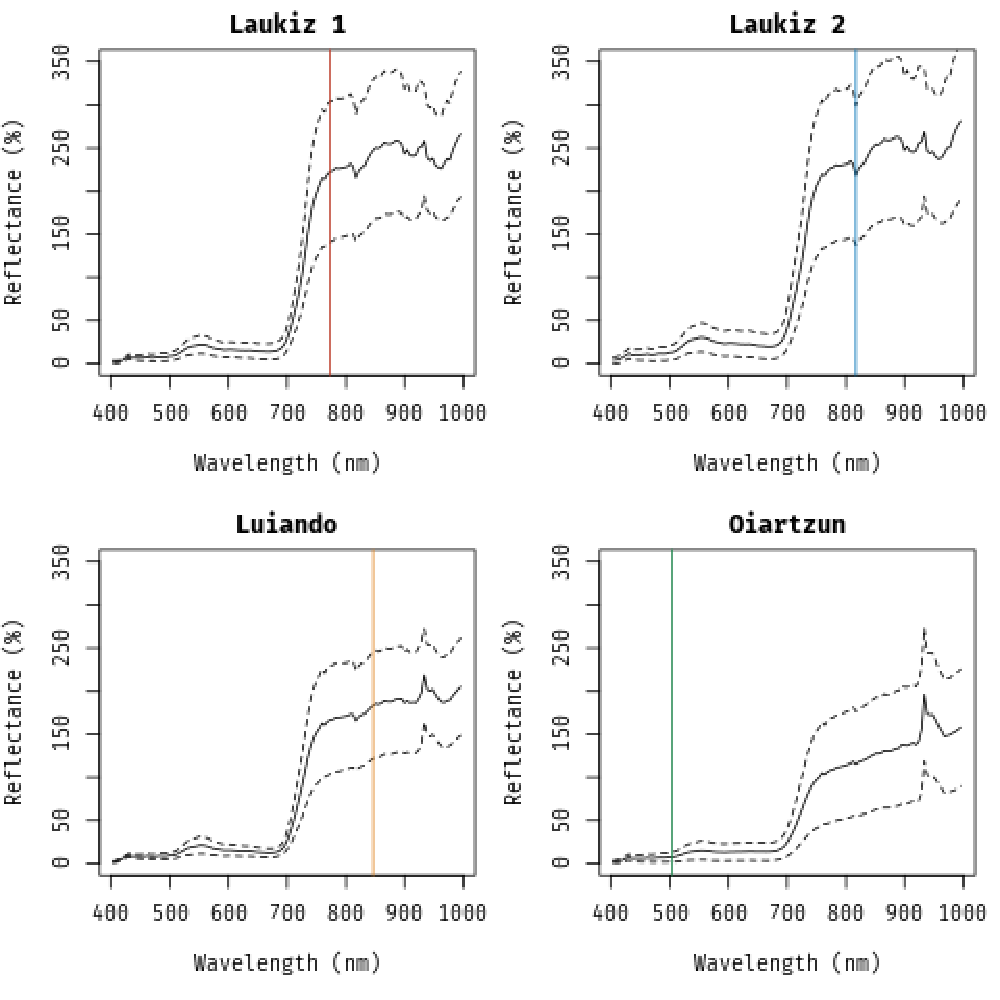
\includegraphics[width=\textwidth] {spectral_signatures.pdf}}
%\caption{Spectral signatures (mean and standard deviation) of each plot.}
%\label{fig:spectral_signatures}
%\end{center}
%\end{figure}

\pagebreak


\section*{References}

\bibliography{Biblio}

\end{document}
